% Template for Elsevier CRC journal article
% version 1.2 dated 09 May 2011

% This file (c) 2009-2011 Elsevier Ltd.  Modifications may be freely made,
% provided the edited file is saved under a different name

% This file contains modifications for Procedia Computer Science

% Changes since version 1.1
% - added "procedia" option compliant with ecrc.sty version 1.2a
%   (makes the layout approximately the same as the Word CRC template)
% - added example for generating copyright line in abstract

%-----------------------------------------------------------------------------------

%% This template uses the elsarticle.cls document class and the extension package ecrc.sty
%% For full documentation on usage of elsarticle.cls, consult the documentation "elsdoc.pdf"
%% Further resources available at http://www.elsevier.com/latex

%-----------------------------------------------------------------------------------

%%%%%%%%%%%%%%%%%%%%%%%%%%%%%%%%%%%%%%%%%%%%%%%%%%%%%%%%%%%%%%
%%%%%%%%%%%%%%%%%%%%%%%%%%%%%%%%%%%%%%%%%%%%%%%%%%%%%%%%%%%%%%
%%                                                          %%
%% Important note on usage                                  %%
%% -----------------------                                  %%
%% This file should normally be compiled with PDFLaTeX      %%
%% Using standard LaTeX should work but may produce clashes %%
%%                                                          %%
%%%%%%%%%%%%%%%%%%%%%%%%%%%%%%%%%%%%%%%%%%%%%%%%%%%%%%%%%%%%%%
%%%%%%%%%%%%%%%%%%%%%%%%%%%%%%%%%%%%%%%%%%%%%%%%%%%%%%%%%%%%%%

%% The '3p' and 'times' class options of elsarticle are used for Elsevier CRC
%% The 'procedia' option causes ecrc to approximate to the Word template
\documentclass[3p,times,procedia]{elsarticle}
\flushbottom

%% The `ecrc' package must be called to make the CRC functionality available
\usepackage{ecrc}
\usepackage[bookmarks=false]{hyperref}
    \hypersetup{colorlinks,
      linkcolor=blue,
      citecolor=blue,
      urlcolor=blue}
%\usepackage{amsmath}


%% The ecrc package defines commands needed for running heads and logos.
%% For running heads, you can set the journal name, the volume, the starting page and the authors

%% set the volume if you know. Otherwise `00'
\volume{00}

%% set the starting page if not 1
\firstpage{1}

%% Give the name of the journal
\journalname{Procedia Computer Science}

%% Give the author list to appear in the running head
%% Example \runauth{C.V. Radhakrishnan et al.}
\runauth{Author name}

%% The choice of journal logo is determined by the \jid and \jnltitlelogo commands.
%% A user-supplied logo with the name <\jid>logo.pdf will be inserted if present.
%% e.g. if \jid{yspmi} the system will look for a file yspmilogo.pdf
%% Otherwise the content of \jnltitlelogo will be set between horizontal lines as a default logo

%% Give the abbreviation of the Journal.
\jid{procs}

%% Give a short journal name for the dummy logo (if needed)
%\jnltitlelogo{Computer Science}

%% Hereafter the template follows `elsarticle'.
%% For more details see the existing template files elsarticle-template-harv.tex and elsarticle-template-num.tex.

%% Elsevier CRC generally uses a numbered reference style
%% For this, the conventions of elsarticle-template-num.tex should be followed (included below)
%% If using BibTeX, use the style file elsarticle-num.bst

%% End of ecrc-specific commands
%%%%%%%%%%%%%%%%%%%%%%%%%%%%%%%%%%%%%%%%%%%%%%%%%%%%%%%%%%%%%%%%%%%%%%%%%%

%% The amssymb package provides various useful mathematical symbols

\usepackage{amssymb}
%% The amsthm package provides extended theorem environments
%% \usepackage{amsthm}

%% The lineno packages adds line numbers. Start line numbering with
%% \begin{linenumbers}, end it with \end{linenumbers}. Or switch it on
%% for the whole article with \linenumbers after \end{frontmatter}.
%% \usepackage{lineno}

%% natbib.sty is loaded by default. However, natbib options can be
%% provided with \biboptions{...} command. Following options are
%% valid:

%%   round  -  round parentheses are used (default)
%%   square -  square brackets are used   [option]
%%   curly  -  curly braces are used      {option}
%%   angle  -  angle brackets are used    <option>
%%   semicolon  -  multiple citations separated by semi-colon
%%   colon  - same as semicolon, an earlier confusion
%%   comma  -  separated by comma
%%   numbers-  selects numerical citations
%%   super  -  numerical citations as superscripts
%%   sort   -  sorts multiple citations according to order in ref. list
%%   sort&compress   -  like sort, but also compresses numerical citations
%%   compress - compresses without sorting
%%
%% \biboptions{authoryear}

% \biboptions{}

% if you have landscape tables
\usepackage[figuresright]{rotating}
%\usepackage{harvard}
% put your own definitions here:x
%   \newcommand{\cZ}{\cal{Z}}
%   \newtheorem{def}{Definition}[section]
%   ...

% add words to TeX's hyphenation exception list
%\hyphenation{author another created financial paper re-commend-ed Post-Script}

% declarations for front matter

\usepackage{float}
\usepackage{amsmath}
\usepackage{booktabs}
\usepackage{array}
\usepackage{tabularx}
\usepackage{enumitem}
\usepackage{hyperref}
\usepackage{graphicx}
\usepackage{url}
\usepackage{microtype}
\usepackage{tikz}
\usetikzlibrary{shapes.geometric,arrows.meta,positioning,calc,fit,backgrounds}
\usepackage{titlesec}
\titlespacing*{\subsection}{0pt}{6pt}{3pt}
\setlength{\parskip}{0pt}
\setlength{\textfloatsep}{4pt plus 1pt minus 1pt}
\setlength{\floatsep}{4pt plus 1pt minus 1pt}
\setlength{\intextsep}{4pt plus 1pt minus 1pt}
\setlength{\abovecaptionskip}{3pt}
\setlength{\belowcaptionskip}{0pt}
\setlist{nosep,leftmargin=*}
\renewcommand{\arraystretch}{0.88}
\AtBeginDocument{%
  \setlength{\abovedisplayskip}{5pt}%
  \setlength{\belowdisplayskip}{5pt}%
  \setlength{\abovedisplayshortskip}{3pt}%
  \setlength{\belowdisplayshortskip}{3pt}%
}

\begin{document}
\begin{frontmatter}

\dochead{International Conference on Machine Learning and Data Engineering}

\title{Real-Time Adaptive Cross-Media Recommendation Using Semantic Embeddings, Knowledge Graph Scoring, and Graph Collaborative Learning}

\author[a]{Sanjay A. K.}
\author[a]{Eswara Raj M.}
\author[a]{Aditya Vijay}
\author[a]{Himaneesh Reddy Jangalapalli}
\author[ca]{Bagavathi Sivakumar P.}
\author[ca]{Krishna Priya G.}

\address[a]{Department of Computer Science and Engineering, Amrita School of Computing, Coimbatore, Amrita Vishwa Vidyapeetham, India}

\begin{abstract}
User preference is inherently spread across various types of media consumed by the user because the same interest can manifest itself as a movie theme, a book topic, an artist of music, a creator search term, a learning purpose and various other types of media. Traditional recommendation systems typically run independently within application silos and hence do not make such connections and do not help the user find different media in the same genre or of the same type. In this paper, we introduce a real-time adaptive cross-media recommendation web application that consolidates movies, books, and music. We do this by removing the boundaries of multi-media interaction by means of a single normalized catalog. Our backend includes Sentence-BERT metadata embeddings, Qdrant approximate nearest neighbors search, deterministic creator-aware search, MySQL-based interactions storage, exponential moving average (EMA) session adaptation, LightGCN collaborative filtering, and in-memory knowledge graph based profile-aware reranking. The React frontend supports profile selection, natural-language search, filters, score-signal display, item details, similar-item retrieval, and feedback.

Our novelty lies in the correspondence among these modules inside one executable pipeline: semantic embeddings handle heterogeneous text and cold start; creator matching protects actor, director, author, and singer queries; EMA reacts to short-term user drift; LightGCN captures collaborative preference; and the knowledge graph connects domains through shared creator, genre, age, profession, and interest entities. Extendable search is achieved by mapping each new domain into the shared schema, after which the same embedding, storage, ranking, API, and frontend flow can be reused. Prototype evaluation over five scenarios reports 5/5 person-match hits for creator queries, 5/5 positive profile-aligned top results in every scenario, average KG proximity of 0.463, average profile alignment of 0.803, and cross-domain output in 60\% of tested scenarios.
\end{abstract}

\begin{keyword}
Recommender systems \sep Cross-media recommendation \sep Sentence-BERT \sep Qdrant \sep LightGCN \sep Semantic search \sep Graph collaborative filtering \sep Real-time personalization \sep Knowledge graph
\end{keyword}

\end{frontmatter}
\textsuperscript{*}Corresponding authors:
\textit{g\_krishnapriya@cb.amrita.edu},
\textit{pbsk@cb.amrita.edu}

\noindent
\textsuperscript{*}Authors:
\textit{cb.sc.u4cse23051@cb.amrita.edu},
\textit{cb.sc.u4cse23022@cb.amrita.edu},
\textit{cb.sc.u4cse23324@cb.amrita.edu},
\textit{cb.sc.u4cse23359@cb.amrita.edu}

\vspace*{-6pt}

\section{Introduction}
\label{sec:introduction}
Recommendation systems are now the main interface through which users discover and explore movies, songs, books, learning resources, and other digital content the users prefer. Most deployed systems widely used presently remain domain-specific: a movie platform recommends films, a music platform recommends tracks, and a book platform recommends books. This separation is practical for platform owners, but it does not reflect how human interest works and how users discover the media they appreciate. A user interested in science fiction may enjoy a film such as \emph{Interstellar}, a novel about space exploration, a soundtrack with similar emotional tone, and educational content on astronomy. A useful recommendation product should connect these signals across media types where recommendations are not bound to any particular media, but a caterer of content based on the preferences of the user across all types of media .

The work described in this paper displays a unified recommendation pipeline for three current domains: movies, books, and music. Each item for all types of media is assigned a common schema with fields such as \texttt{global\_id}, \texttt{content\_type}, title, description, creator information, category, release date, popularity, rating, metadata and embedding text. This representation allows heterogeneous datasets to be indexed in one semantic retrieval layer where each media item across domains is represented as an entity. On top of this, the system logs and tracks user interactions and uses both immediate and periodically trained methods go show personalization. The goal is not only to retrieve semantically similar content, but also to merge it with recommendations adapted to user behavior and trends over time.

Three technical directions have motivated the implementation. Sentence-BERT enables the comparison of items using the descriptions of the item across domains \cite{reimers2019sbert}; LightGCN learns from user-item interaction graphs over time \cite{he2020lightgcn}; and Qdrant supports low-latency nearest-neighbor retrieval \cite{qdrant}. The implemented FastAPI \cite{fastapi} backend integrates Qdrant for retrieval, MySQL for data storage and logging, PyTorch LightGCN for reranking, EMA for adapting to user sessions, and an in-memory knowledge graph for entity-aware profile scoring.

The key research gap is that these capabilities are rarely implemented together in a single functioning multi-domain product pipeline. Graph-based models are often used as a benchmark on single-domain interaction datasets; Semantic systems retrieve content based on meaning and similarity rather than the user's preferences; cross-domain approaches commonly move between two domains instead of normalizing several domains into one catalog; and real-time personalization is often treated independently from graph learning.

The design addresses heterogeneous metadata from various media, item cold start problem, session-level preference drift, hybrid-score fusion, people-based search over actors/directors/authors/singers, and age/profession-aware scoring without private social data.

Contributions are purposely kept brief and focused on three key points:
\begin{enumerate}
    \item An integrated movie, book, and music platform that supports semantic, creator-aware, and flexible search through a unified catalog and web application.

    \item A combined ranking model using Sentence-BERT/Qdrant retriever, EMA-based personalization, LightGCN graph scoring, and Knowledge Graph profile scoring.

    \item  A system evaluated both mathematically and through a working prototype, showing quantitative and qualitative improvements over conventional single-signal recommenders.
\end{enumerate}

\section{Discussion of Related Work and Novelty}
\label{sec:discussion}
Methods used to recommend include Collaborative Filtering, Content-Based Recommendations, Hybrid Recommendations,
Graph Neural Collaborative Filtering, Semantic Retrieval, Knowledge-Graph Recommendation, Adaptive Approaches, and
Cross-Domain Transfer. Collaborative Filtering is based on behavior, content-based recommendations on meta data, while hybrid
approaches combine them to curtail the cold start problem .\cite{zhang2019deep}.
Neural Graph Collaborative Filtering (NGCF) uses the graph convolution to based user–item relationships, but what LightGCN does it simplifies this method by erasing the feature transformations and the nonlinear activation functions, and focus instead on efficient neighborhood-based embedding propagation.\cite{wang2019ngcf,he2020lightgcn}.So here the LightGCN is used as the collaborative reranking mechanism instead of initial candidate-generation mechanism. Semantic retrival initially finds relevant cross-media candidates, after which the graph-derived representations gives an additional signal for users who has enough interaction history.The sequential recommendation method i.e SASRec models the order of user actions and that are commonly evaluated in domain-specific offline  settings \cite{kangg2018sasrec};this performs a differnent role from the cross media , the hybrid ranking pipeline approach is choosen in this area.

Semantic embedding methods compute item similarity even before a considerable amount of user interactions exist. Sentence-BERT is practical because it produces sentence embeddings comparable by cosine similarity \cite{reimers2019sbert}. Here, each item is converted into embedding text by combining title, categories, description, and creator information, placing movies, books, and songs in a shared vector space.

Knowledge graph systems such as KGAT and RippleNet connect users, items, and entities through relations such as acted-in, directed-by, written-by, and belongs-to-genre \cite{wang2019kgat,wang2018ripplenet}. The current implementation uses an in-memory KG from the unified catalog for entity-proximity scoring. cross domain research supports preference transfer between domains, although many works still focus on two-domain transfer \cite{zang2022cross}; a recent comprehensive survey has begun to broaden this scope to multi-domain and task-guided transfer settings \cite{zhang2025survey}. Large language models augmented with graph structure have also recently been explored as an alternative route to relevance and explanation generation \cite{wu2024llmrec}.

So recently the studies from Amrita Vishwa Vidyapeetham have investigated that several of the recommendation system have challenges including the import cold start prediction , optimizing collaborative filtering , sparse interaction data, the dual feedback personalization, and the community aware recommendation \cite{amrita2023densenet,amrita2023adamvrgo,amrita2024sparse,
amrita2025dualfeedback,amrita2026svd}. So these studies the primarily address the integration of the heterogeneous media into the common recommendation pipeline. Movies , books and music are represented using the same catalog schema and processed through shared retrieval , personalization , and reranking stages . So the distinction of the proposed architecture system is the cross media integration rather than in introducing another standalone model.


The novelty of this work is not a new neural layer; it is the applied correspondence of mature methods using one working product pipeline. Sentence-BERT corresponds to cross-domain semantic understanding, Qdrant to low-latency vector retrieval, MySQL to durable interaction memory, EMA to instant preference drift handling, LightGCN to collaborative preference propagation, and the knowledge graph to entity/profile reasoning. Relative systems usually emphasize one of these capabilities. The proposed system combines all of them while preserving a clear input-output API and a domain-extension path.
Different from a traditional hybrid recommendation system. This system scores from both the content and the collaborative filters after training in separate domains, it starts by mapping heterogeneous media data to one common schema for vector searches, creator lookups, graphs building, API responses, and frontend presentations. Cross-media recommendation is therefore treated as both a data-modeling problem and a ranking problem.The system also separates immediate and delayed personalization. EMA reacts after a single like, skip, or bookmark, while LightGCN is refreshed after enough interactions accumulate. This division is practical because sessions change periodically but graph training is more expensive.

\begin{table}[t]
\centering
\caption{Comparison of prior model families, common measures, and implemented signals. Each row maps a family of prior work to the measures it is normally evaluated with and to the corresponding sub-score computed inside the proposed pipeline.}
\label{tab:metricmap}
\footnotesize
\begin{tabularx}{\linewidth}{p{0.22\linewidth}p{0.29\linewidth}p{0.23\linewidth}X}
\toprule
Family & Common measures in papers & Typical limitation & Correspondence in this work \\
\midrule
Semantic/content recommenders & Precision@K, Recall@K, similarity, coverage & weak collaborative behaviour & $S_{\mathit{sem}}$, cold-start retrieval, cross-domain coverage. \\
Graph collaborative models & HitRate@K, NDCG@K, MRR, BPR loss & sparse cold start and single-domain focus & $S_{\mathit{graph}}$, positive interaction graph, holdout-ready LightGCN. \\
KG recommenders & entity relevance, explainability, Recall@K/NDCG@K & graph construction cost & $S_{\mathit{kg}}$, creator/genre/profile entity overlap. \\
Online systems & latency, click response, session adaptation & difficult streaming retraining & EMA update and immediate profile-aligned reranking. \\
Hybrid systems & accuracy, diversity, coverage, satisfaction & complex score calibration & weighted final score with visible sub-signals. \\
\bottomrule
\end{tabularx}
\end{table}

Table~\ref{tab:metricmap} also addresses metric compatibility with existing papers. Precision@K, Recall@K, NDCG@K, MRR, and MAP are standard for labelled offline relevance benchmarks, especially MovieLens, Amazon-Book, Yelp, and Gowalla-style datasets. The present dataset contains prototype interactions rather than a large public relevance benchmark, so this paper reports implementation-level measures that can be directly computed from the available catalog and profiles: PersonHit@5, ProfileAlign@5, KG proximity, profile score, and DomainCoverage@10. The final score is therefore aligned with pre-existing recommender measures, but not presented as a replacement for full benchmark evaluation.

\section{Implementation}
\label{sec:implementation}
\subsection{Web application system}
The implemented system is a modular web recommendation product. The frontend provides user profile selection, natural-language search, content-type filters, recommendation cards, score-signal display, detail views, similar-item search, and interaction buttons. The backend exposes recommendation and interaction APIs. The data pipeline preprocesses heterogeneous datasets into a common catalog, generates embeddings, uploads vectors to Qdrant, stores content and user interactions in MySQL, trains LightGCN artifacts from positive interaction logs, and exposes KG-profile scoring at query time.

The web application request flow begins when the user enters a query such as \texttt{space adventure with aliens}, \texttt{James Cameron}, or \texttt{business analytics and learning}. The request contains the query, optional user ID, optional content-type filter, and desired top-$K$. The backend validates the request using Pydantic, checks direct creator matches, embeds the query, retrieves vector candidates from Qdrant, applies optional MySQL-backed personalization, blends all scores, and returns JSON results.Finally, on the frontend we have titles, domain, creators, categories, score bars, and the ability to provide feedback.
User feedback is returned to the backend and used in further ranking.

\begin{figure}[t]
    \centering
    \includegraphics[width=0.8\textwidth]{chad.png}
    \caption{System architecture. The diagram separates the retrieval layer (Sentence-BERT encoding and Qdrant approximate nearest-neighbor search), the storage layer (MySQL catalog and interaction logs), the personalization layer (EMA session updates and periodically retrained LightGCN embeddings), and the presentation layer (FastAPI endpoints consumed by the React frontend), with arrows indicating request-time versus training-time data flow.}
    \label{fig:architecture}
\end{figure}

Figure~\ref{fig:architecture}retrieval, storage, personalization, and presentation are separated such that each component may be tested separately.
Qdrant search occurs during request time, EMA updates right after feedback, and LightGCN can be retrained periodically.
The system generates clear intermediate artifacts: normalized catalog rows, embedded text, dense vectors, Qdrant payloads, interaction logs for MySQL, and exported graph embeddings.
This flow of artifacts makes experiments more reproducible since errors could be pinpointed to one step rather than being hidden in one end-to-end model.


\subsection{Data sources and unified catalog}
Probably the key decision in the implementation was to translate all domains to one unified schema.
Movies use TMDb movie metadata and credits \cite{tmdb},  books use a dataset similar to Google Books with optional enrichment through Open Library APIs\cite{openlibrary}, and music uses Kaggle songs dataset with optional enrichment through MusicBrainz API\cite{musicbrainz}. Common fields are \texttt{global\_id}, \texttt{content\_type}, \texttt{source\_id}, \texttt{title}, \texttt{description}, \texttt{creators}, \texttt{categories}, \texttt{release\_date}, \texttt{popularity}, \texttt{rating}, \texttt{metadata\_text}, \texttt{embedding\_text}, and \texttt{text\_hash}.

In the case of movies, the pre-processing phase combines titles, overviews, genres, keywords, directors, and the main cast. In case of books we take the author field and it is mapped into the shared \texttt{creators} column, while categories and descriptions are taken in as semantic text. For music, track artist and album information is mapped into \texttt{creators} and metadata fields. It allows the same search logic to handle actors, directors, authors, and singers. The \texttt{text in the metadata} field \ is the richer text used for inspection and storage, while \texttt{the embedding \_text} is a clean natural-language string used for model encoding. SHA-256 text hash allows to reuse embeddings from previous
build in case embedding text field of a row was not modified. The catalog is separated source identity
from global identity to prevent collision of raw ids from different datasets.

The catalog separates the source identity from a global identity so raw IDs from different datasets do not collide with it. The \texttt{content\_type} field becomes the domain switch used by filters, API responses, KG nodes, and frontend badges. Ratings and popularity remain optional, keeping the schema robust when new domains are added.

Extendable search means that a new domain does not require a new recommender pipeline. Let each domain $d \in \mathcal{D}$ provide a mapper $\phi_d(x)$ from a raw row $x$ into the shared item representation $r_i$. The catalog is
\begin{equation}
    \mathcal{C}=\bigcup_{d\in\mathcal{D}}\{\phi_d(x):x\in X_d\},
    \quad
    r_i=(id,type,title,desc,creators,categories,text_i).
    \label{eq:catalog_union}
\end{equation}
When a fourth domain such as courses, podcasts, games, or short videos is added, only $\phi_d$ must be defined; embedding, vector search, KG scoring, API response, and frontend rendering remain unchanged.

\subsection{Semantic embedding and vector search}
The semantic retrieval layer uses Sentence-BERT, specifically the compact \texttt{all-MiniLM-L6-v2} model, to convert item metadata into dense 384-dimensional vectors \cite{reimers2019sbert}. This 384-dimensional size is fixed by the output layer of \texttt{all-MiniLM-L6-v2} rather than a free hyperparameter of the system; keeping item embeddings, the query embedding, and the user profile vector (Section~\ref{sec:ema}) in this same space is what allows cosine similarity to be computed directly between users, items, and queries without an extra projection layer. The embedding text for each item is formed by concatenating title, categories, description, and creator information into a single natural-language string. Let $\mathbf{e}_i \in \mathbb{R}^{384}$ be the embedding of item $i$ and $\mathbf{q} \in \mathbb{R}^{384}$ be the encoded query. The semantic similarity score is
\begin{equation}
    S_{\mathit{sem}}(i,q)=
    \frac{\mathbf{e}_i^\top \mathbf{q}}{\|\mathbf{e}_i\|\,\|\mathbf{q}\|}.
    \label{eq:cosine}
\end{equation}
At retrieval time, Qdrant uses this cosine distance function to conduct approximate nearest neighbor search and retrieves top-K
results along with the scores. Content-type filtering is an optional functionality that the backend offers so that users can choose to search
all domains or only one such as movies, books, or music. As the item payload information is available in Qdrant, all the required
information such as title, description, creator names, categories, popularity, rating, and score is provided within one API request.

The semantic layer is responsible for enabling cold start and cross-domain retrieval as a new item can be recommended based on its
metadata without any interaction while the same query can retrieve movie, book, or song whose metadata is semantically similar.

Vector-based search is employed for candidate generation and not the final ranking. Qdrant fast retrieves semantically similar
items whereas the reranking phase takes care of user preference, creator intent, graph information, and KG/Profile relevance.

\subsection{Person-aware search over creators}
The challenge with recommendation interfaces is that most people tend to search for persons and not topics. Vector
search alone does not distinguish between names and generic text and will likely skip the exact match in the catalog.
Thus, the backend tries to find an exact match, prefix match, and substring match of normalized creators before semantic
searching. At most, five items directly related to a person get sorted first, and semantic items are added to the list
after the global id deduplication process.
The reason why this is important is that intent behind names is not always represented through dense similarity. If
people search for James Cameron, then films related to him should be prioritized. On the other hand, if someone searches
for Taylor Swift, then only her music and no duplicates should be returned, but cross-media hits are possible where
metadata allows. The common creators field is both the search field and a source of the graph entities.
Searching for creators is deterministic: exact matches have the highest priority, prefixes second and substrings last.

\subsection{Interaction logging and EMA adaptation}
\label{sec:ema}
The backend records user interactions through a dedicated API. Supported event types include \texttt{view}, \texttt{click}, \texttt{like}, \texttt{bookmark}, \texttt{rating}, \texttt{skip}, and \texttt{complete}. These events are stored in MySQL and used for personalization. Positive events such as likes, bookmarks, completions, and high ratings pull the user's vector toward the content embedding; negative events such as skips push it away.

Let $\mathbf{u}_t \in \mathbb{R}^{384}$ be the current user profile vector -- kept in the same 384-dimensional Sentence-BERT space as the item embeddings so that $\mathbf{u}_t$ and $\mathbf{e}_i$ remain directly comparable by cosine similarity -- $\mathbf{e}_i$ be the embedding of the interacted item, and $\alpha \in (0,1)$ be the smoothing factor. For a positive event, the profile update is
\begin{equation}
    \mathbf{u}_{t+1}=\alpha\mathbf{e}_i+(1-\alpha)\mathbf{u}_t.
    \label{eq:ema_update}
\end{equation}
The EMA score assigned to a candidate item $i$ is
\begin{equation}
    S_{\mathit{ema}}(i,u)=
    \frac{\mathbf{e}_i^\top\mathbf{u}_t}{\|\mathbf{e}_i\|\,\|\mathbf{u}_t\|}.
    \label{eq:ema_score}
\end{equation}
EMA enables lightweight real-time adaptation without retraining the graph model after every click. It is therefore useful for session-level changes such as a user temporarily moving from entertainment queries to learning queries.

The choice of EMA is intentionally simple. More complex online learning can update model parameters continuously, but EMA updates only a user vector and is cheap enough for every event. Likes move $\mathbf{u}_t$ toward preferred semantic regions; skips move it away, and the resulting score blends with semantic and graph scores without changing item vectors.

\subsection{Graph collaborative filtering with LightGCN}
Semantic retrieval explains item similarity but not collaborative behaviour. The system therefore includes a PyTorch LightGCN module trained on positive MySQL user-item interactions; exported user and item embeddings are used for backend reranking.

LightGCN represents users and items as nodes in a bipartite interaction graph $\mathcal{G}=(\mathcal{U}\cup\mathcal{I},\mathcal{E})$, where each edge $(u,i)\in\mathcal{E}$ corresponds to a positive interaction. Let $\mathbf{e}^{(0)}_u$ and $\mathbf{e}^{(0)}_i$ be the initial learnable embeddings. The $\ell$-th layer propagation rule is
\begin{equation}
    \mathbf{e}^{(\ell)}_u =
    \sum_{i\in\mathcal{N}_u}
    \frac{\mathbf{e}^{(\ell-1)}_i}{\sqrt{|\mathcal{N}_u|}\sqrt{|\mathcal{N}_i|}},
    \quad
    \mathbf{e}^{(\ell)}_i =
    \sum_{u\in\mathcal{N}_i}
    \frac{\mathbf{e}^{(\ell-1)}_u}{\sqrt{|\mathcal{N}_i|}\sqrt{|\mathcal{N}_u|}}.
    \label{eq:lightgcn_prop}
\end{equation}
After $L$ propagation layers, the final embedding is the mean over all layers:
\begin{equation}
    \mathbf{e}_u=\frac{1}{L+1}\sum_{\ell=0}^{L}\mathbf{e}^{(\ell)}_u,
    \quad
    \mathbf{e}_i=\frac{1}{L+1}\sum_{\ell=0}^{L}\mathbf{e}^{(\ell)}_i.
    \label{eq:lightgcn_avg}
\end{equation}
This is the trained (BPR)Bayesian Personalized Ranking loss equation:
\begin{equation}
    \mathcal{L}_{\mathrm{BPR}}=
    -\sum_{(u,i,j)\in\mathcal{D}}\ln\sigma(\hat{y}_{ui}-\hat{y}_{uj})
    +\lambda\|\Theta\|^2,
    \label{eq:bpr}
\end{equation}
here $\hat{y}_{ui}=\mathbf{e}_u^\top\mathbf{e}_i$ and $j$ is a sampled negative item. BPR is used instead of a pointwise loss such as mean-squared error or binary cross-entropy because the available signal is implicit and positive-only -- views, likes, bookmarks, and completions -- with no reliable explicit negative label for an item a user has simply not seen. Rather than asking the model to predict an absolute score for each interaction, BPR contrasts every observed positive interaction against a sampled unobserved item and directly optimizes the pairwise ranking order that the recommender needs at inference time, which is also why it is the standard training objective for LightGCN and most graph collaborative filtering models trained on implicit feedback \cite{he2020lightgcn,wang2019ngcf}. At inference time, the graph compatibility score is
\begin{equation}
    S_{\mathit{graph}}(i,u)=\mathbf{e}_u^\top\mathbf{e}_i.
    \label{eq:graph_score}
\end{equation}

The graph stage is a reranker rather than a candidate generator. Semantic retrieval supports cold-start discovery, while LightGCN is strongest when both user and item appear in the interaction graph. If a graph score is unavailable, the candidate can still be ranked using semantic, EMA, KG, and profile signals.

\subsection{Knowledge graph and profile-aware scoring}
The system includes an in-memory knowledge graph built directly from the processed catalog. Instead of requiring a separate graph database at this stage, the KG derives entity signals from content type, title, categories, creators, descriptions, and user profile metadata. The practical node types are \emph{User}, \emph{Movie}, \emph{Book}, \emph{Song}, \emph{Creator}, \emph{Genre}, \emph{Profession}, \emph{Age Group}, and \emph{Interest/Skill}. Practical relations include \texttt{liked}, \texttt{bookmarked}, \texttt{completed}, \texttt{belongs\_to\_genre}, \texttt{directed\_by}, \texttt{written\_by}, \texttt{performed\_by}, \texttt{suitable\_for}, and \texttt{related\_to\_profession}. Figure~\ref{fig:knowledge_graph} illustrates the resulting entity graph and shows how a preference path can move from a user, through a shared creator, genre, age, or profession entity, into an item of a different media type.

\begin{figure*}[t]
    \centering
    \includegraphics[width=0.8\textwidth]{di.png}
    \caption{Knowledge graph representation used for user profiling and cross-media recommendation. User, Movie, Book, Song, Creator, Genre, Profession, Age Group, and Interest/Skill nodes are connected through relations such as \texttt{liked}, \texttt{directed\_by}, \texttt{written\_by}, \texttt{performed\_by}, and \texttt{related\_to\_profession}; because creator, genre, and profile entities are shared across domains, a path leaving a user node can arrive at a movie, book, or song node without a domain-specific edge.}
    \label{fig:knowledge_graph}
\end{figure*}

Multi-domain reasoning works because relation paths can cross media boundaries through shared entities:
\begin{equation}
    P(u,i)=\{u\rightarrow e_1\rightarrow\cdots\rightarrow i:
    e_k\in \mathcal{E}_{creator}\cup\mathcal{E}_{genre}\cup\mathcal{E}_{profile}\}.
    \label{eq:paths}
\end{equation}
For example, a science-fiction movie preference can move through a genre node to space-themed books or songs; a data analyst profile can move through profession nodes to analytics, business, technology, and learning content across domains.

The KG score measures how closely query terms overlap with the entity tokens of a candidate item. Let $\mathcal{T}(q)$ be the token set derived from query $q$ and $\mathcal{T}(i)$ be the combined token set of item $i$'s title, description, creators, categories, and content type. The proximity score is
\begin{equation}
    S_{\mathit{kg}}(i,q)=
    \min\!\left(1,\frac{|\mathcal{T}(q)\cap\mathcal{T}(i)|}
    {\max(3,|\mathcal{T}(q)|)}\right).
    \label{eq:kg_score}
\end{equation}
The profile score rewards items that align with the user's declared age group, profession, interests, and skills, while penalizing categories flagged as unsuitable:
\begin{equation}
    S_{\mathit{profile}}(i,u)=
    \sum_{t\in\mathcal{P}_{+}(u)} \delta(t,i)w_{+}
    -\sum_{t\in\mathcal{P}_{-}(u)} \delta(t,i)w_{-}
    +\mathbf{1}[\mathrm{pref}(u)=\mathrm{type}(i)]w_c.
    \label{eq:profile_score}
\end{equation}
Here $\delta(t,i)=1$ if term $t$ appears in item $i$, $w_+=0.16$, $w_-=0.25$, and $w_c=0.15$. The final score is clipped to $[-1,1]$. This profile design intentionally avoids private social-media scraping and uses declared, consent-based profile attributes.

The KG is multi-domain because it does not create separate movie, book, and music graphs. All domains use shared entity namespaces: creators, genres, topics, profiles, ages, professions, and interests. The recommender can move from a user profile to an entity and then to any item type sharing that entity, giving a structured bridge beyond dense-vector similarity.

\subsection{Recommendation pipeline and algorithms}
The recommendation pipeline is an ordered algorithm rather than a single monolithic model. Given $(q,u,K,type)$, the backend validates the request, normalizes the query/domain filter, reserves exact creator matches when available, embeds the query with Sentence-BERT, retrieves Qdrant candidates, removes duplicates, applies optional type filtering, adds EMA/LightGCN/KG/profile scores when user context is available, and sorts by the hybrid score:
\begin{equation}
    S(i,u,q)=S_{\mathit{sem}}(i,q)+
    \lambda_gS_{\mathit{graph}}(i,u)+
    \lambda_eS_{\mathit{ema}}(i,u)+
    \lambda_kS_{\mathit{kg}}(i,q)+
    \lambda_pS_{\mathit{profile}}(i,u).
    \label{eq:hybrid}
\end{equation}
The implementation uses $\lambda_g=0.20$, $\lambda_e=0.15$, $\lambda_k=0.08$, and $\lambda_p=0.10$ as tunable blending weights. The output is a ranked list $R_u=[i_1,i_2,\ldots,i_K]$ sorted by decreasing $S(i,u,q)$, with metadata and score signals returned to the frontend.

The algorithm therefore treats the input both as free text and as possible creator intent. High-confidence name matches are preserved, Qdrant supplies broad candidates, user-specific signals are added only for known profiles, and bounded sub-scores are returned so the frontend can display signal explanations.

\subsection{Backend API and frontend integration}
The backend is implemented using FastAPI with Pydantic validation and OpenAPI documentation \cite{fastapi}. The main endpoints are \texttt{GET /health}, \texttt{GET /search/suggest}, \texttt{POST /recommend}, \texttt{POST /recommend/item}, \texttt{POST /interactions}, and \texttt{GET /interactions/\{user\}/\{item\}}.

The React frontend provides demo profile login, natural-language search, filters, result cards, score-signal display, similar-item search, detail modal, and feedback controls. It turns the backend into an interactive product prototype where feedback events immediately affect later recommendations through EMA.

The API response is transparent: each recommendation contains metadata, final score, and optional sub-scores. A simplified response item is
\[
    (id,type,title,creators,categories,S,S_{\mathit{sem}},S_{\mathit{graph}},
    S_{\mathit{ema}},S_{\mathit{kg}},S_{\mathit{profile}}).
\]
Visible score bars can therefore show whether a recommendation was driven mainly by semantic similarity, graph compatibility, EMA adaptation, or KG/profile alignment. Table~\ref{tab:modules} summarizes each pipeline stage, its input and output, and the algorithm or technology used, providing a compact map from raw catalog rows to this final JSON response.

\begin{table}[t]
\centering
\caption{Module-wise input, output, algorithm, and implementation technology. Each row corresponds to one stage of the pipeline described in Section~\ref{sec:implementation}, read top to bottom in execution order from raw dataset ingestion to the JSON response consumed by the frontend.}
\label{tab:modules}
\footnotesize
\begin{tabularx}{\linewidth}{p{0.20\linewidth}p{0.18\linewidth}p{0.22\linewidth}X}
\toprule
Module & Input & Algorithm / technology & Output \\
\midrule
Preprocessing & raw movie/book/music rows & Pandas schema mapper $\phi_d$ & unified catalog and embedding text \\
Semantic retrieval & query and metadata text & Sentence-BERT + cosine + Qdrant ANN & top-$K$ semantic candidates \\
Creator search & person-name query & exact/prefix/substring matching & actor/director/author/singer hits \\
Interaction memory & feedback event & MySQL logging & user-item history \\
Real-time adaptation & user vector and item vector & EMA update & session-aware user profile vector \\
Graph learning & positive interactions & LightGCN with BPR loss & user/item collaborative embeddings \\
KG/profile scoring & query, item, profile & entity overlap and profile weights & KG and profile sub-scores \\
API/frontend & request and ranked list & FastAPI + React & JSON response and interactive UI \\
\bottomrule
\end{tabularx}
\end{table}

\section{Results}
\label{sec:results}
Five exemplary scenarios were considered from the catalog and demo profiles:
actor/director search, singer/artist search, profession-sensitive learning, family-friendly recommendations, and cross-media
semantic intent. Quantitative metrics include PersonHit@5, ProfileAlign@5, average KG proximity, average profile score, and
DomainCoverage@10. Qualitative inspection tests if the best results are comprehensible, if the exact person queries are
followed, if the unwanted categories are lessened, and if the general intent allows multiple domains.

\begin{table}[t]
\centering
\caption{Prototype results and comparison with relative single-signal systems. The top block compares the hybrid pipeline's averages against relative semantic-only, graph-only, and KG/profile-only baselines; the bottom block gives the per-scenario measures, and the rightmost column names the media domains present in that scenario's top-10 results.}
\label{tab:results}
\footnotesize
\begin{tabularx}{\linewidth}{p{0.25\linewidth}p{0.14\linewidth}p{0.15\linewidth}p{0.09\linewidth}p{0.11\linewidth}X}
\toprule
System / scenario & PersonHit@5 & ProfileAlign@5 & Avg. KG & Avg. profile & Domains@10 \\
\midrule
Semantic-only relative system & -- & -- & limited & limited & text-dependent \\
Graph-only relative system & -- & interaction-dependent & -- & -- & sparse cold start \\
KG/profile-only relative system & creator/entity-aware & profile-aware & yes & yes & no collaborative signal \\
\textbf{Proposed hybrid average} & \textbf{1.00 person queries} & \textbf{1.00} & \textbf{0.463} & \textbf{0.803} & \textbf{0.60} \\
\midrule
James Cameron / sci-fi & 5/5 & 5/5 & 0.467 & 0.990 & movie \\
Taylor Swift / pop & 5/5 & 5/5 & 0.667 & 0.694 & movie,music \\
Business analytics & 0/5 & 5/5 & 0.250 & 0.446 & book,movie \\
Family animation & 0/5 & 5/5 & 0.533 & 0.884 & movie \\
Space adventure & 0/5 & 5/5 & 0.400 & 1.000 & book,movie \\
\bottomrule
\end{tabularx}
\end{table}

Table~\ref{tab:results} present all these metrics for each of the five scenarios and at the very to  block, compares the proposed hybrid average against relative semantic-only, graph-only, and KG/profile-only baselines that each expose only one of the implemented signals.

\begin{figure}[t]
\centering
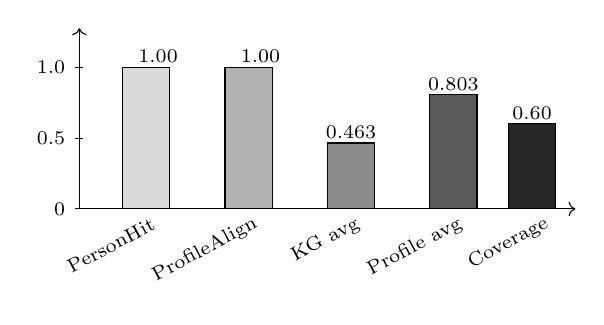
\begin{tikzpicture}[font=\scriptsize, yscale=0.9]
\draw[->] (0,0) -- (6.3,0);
\draw[->] (0,0) -- (0,2.55);
\foreach \y/\lab in {0/0,1/0.5,2/1.0}{\draw (-0.05,\y) -- (0.05,\y) node[left=3pt]{\lab};}
\draw[fill=black!15] (0.55,0) rectangle (1.15,2.00);
\draw[fill=black!30] (1.85,0) rectangle (2.45,2.00);
\draw[fill=black!45] (3.15,0) rectangle (3.75,0.93);
\draw[fill=black!65] (4.45,0) rectangle (5.05,1.61);
\draw[fill=black!85] (5.45,0) rectangle (6.05,1.20);
\node[rotate=28,anchor=east] at (1.05,-0.13) {PersonHit};
\node[rotate=28,anchor=east] at (2.35,-0.13) {ProfileAlign};
\node[rotate=28,anchor=east] at (3.65,-0.13) {KG avg};
\node[rotate=28,anchor=east] at (4.95,-0.13) {Profile avg};
\node[rotate=28,anchor=east] at (6.05,-0.13) {Coverage};
\node at (1.0,2.15) {1.00};
\node at (2.3,2.15) {1.00};
\node at (3.45,1.08) {0.463};
\node at (4.75,1.76) {0.803};
\node at (5.75,1.35) {0.60};
\end{tikzpicture}
\caption{Black-and-white result graph with five normalized comparison metrics -- PersonHit@5, ProfileAlign@5, average KG proximity, average profile score, and DomainCoverage@10 -- each averaged across the five evaluation scenarios of Table~\ref{tab:results} and plotted on a common 0--1 scale for quick visual comparison.}
\label{fig:results}
\end{figure}

Figure~\ref{fig:results} visualizes the five aggregate metrics from Table 3 on the common 0 to 1 scale and demonstrates how
person-query precision and profile alignment achieve their maximum value, while KG proximity and cross-domain coverage stay the more conservative
signals as expected due to their strict overlap-based definitions in Equations~\eqref{eq:kg_score} and \eqref{eq:profile_score}.

The results reveal the novelty connection: semantic search provides general cross-media candidates, while exact
creator matching and KG/profile re-ranking increase understandability and alignment. The strongest qualitative outputs were \emph{Avatar} for \texttt{James Cameron}, \emph{Lover (Remix)} for \texttt{Taylor Swift}, \emph{Minions} for family animation, and \emph{Interstellar} for space-adventure intent.

These scenarios test different components of the architecture: deterministic creator search, profession/skill reranking,
family-friendly profile alignment, and cross-media semantics distribution. The scenarios are not intended to substitute a public benchmark but only to verify the fact that the final score does not represent semantic similarity under a different name.
The metrics correspond to existing evaluation classes on a prototypical level: PersonHit@5 is precision-like for creator queries; ProfileAlign@5 is a top-$K$ relevance metric for profile suitability; KG proximity is an entity relevance metric;
profile score is a suitability metric; and DomainCoverage@10 is a cross-media spread metric. Proper benchmarking with Recall@K, NDCG@K, MAP, MRR, diversity, and latency are future work because of the need for more labelled data.

\section{Conclusion and Future Work}
\label{sec:conclusion}
The papaer is described as a real-time adaptive cross-media recommendation engine using unified catalog,
Sentence-BERT embeddings, Qdrant vector search, MySQL interaction logging, EMA personalization, LightGCN
collaborative filtering, in-memory knowledge graph, FastAPI services, and React user interface. Final hybrid ranking is done
on the basis of semantic similarity, graph compatibility, EMA profile similarity, KG entity similarity, and age/profession
profile match.
The paper explains how movies, books, and music can be searched using one extensible schema but still allowing for
person-specific searching over actors, directors, authors, and singers. Cross-media recommendation is done by leveraging
common entities: creator, genre, profile, age group, profession, interest, and interaction history. Prototype results show high
person-query precision, profile matching, KG/profile score, and multiple domain output.
There are still limitations in the prototype: metadata quality is dependent on dataset available, LightGCN is trained in
prototype size, KG is based on in-memory implementation, and multimodal embeddings, fairness/diversity reranking,
and production latency benchmarking are missing. Future work will improve metadata via official APIs, will implement
KG in graph database, will add more domains like courses, podcasts, run Recall@K/NDCG@K/MRR/MAP evaluation, and conduct user studies.

\vspace{-6pt}

\begin{thebibliography}{00}
\linespread{1.4}\scriptsize
\setlength{\itemsep}{0pt}
\setlength{\parskip}{0pt}
\setlength{\parsep}{0pt}
\setlength{\topsep}{0pt}

\bibitem{wang2019ngcf}
X. Wang, X. He, M. Wang, F. Feng, and T.-S. Chua, ``Neural graph collaborative filtering,'' in \emph{Proc. 42nd International ACM SIGIR Conference on Research and Development in Information Retrieval}, 2019, pp. 165--174.

\bibitem{he2020lightgcn}
X. He, K. Deng, X. Wang, Y. Li, Y. Zhang, and M. Wang, ``LightGCN: Simplifying and powering graph convolution network for recommendation,'' in \emph{Proc. 43rd International ACM SIGIR Conference on Research and Development in Information Retrieval}, 2020, pp. 639--648.

\bibitem{reimers2019sbert}
N. Reimers and I. Gurevych, ``Sentence-BERT: Sentence embeddings using Siamese BERT-networks,'' in \emph{Proc. EMNLP-IJCNLP}, 2019, pp. 3982--3992.

\bibitem{kang2018sasrec}
W.-C. Kang and J. McAuley, ``Self-attentive sequential recommendation,'' in \emph{Proc. IEEE International Conference on Data Mining}, 2018, pp. 197--206.

\bibitem{zang2022cross}
T. Zang, Y. Zhu, H. Liu, R. Zhang, and J. Yu, ``A survey on cross-domain recommendation: Taxonomies, methods, and future directions,'' \emph{ACM Transactions on Information Systems}, vol. 41, no. 2, 2022.

\bibitem{wang2019kgat}
X. Wang, X. He, Y. Cao, M. Liu, and T.-S Chua, ``KGAT: Knowledge graph attention network for recommendation,'' in \emph{Proc. 25th ACM SIGKDD Conference on Knowledge Discovery and Data Mining}, 2019, pp. 950--958.

\bibitem{wang2018ripplenet}
H. Wang et al., ``RippleNet: Propagating user preferences on the knowledge graph for recommender systems,'' in \emph{Proc. 27th ACM International Conference on Information and Knowledge Management}, 2018, pp. 417--426.

\bibitem{wu2024llmrec}
L. Wu et al., ``LLMRec: Large language models with graph augmentation for recommendation,'' in \emph{Proc. 17th ACM International Conference on Web Search and Data Mining}, 2024, pp. 806--815.

\bibitem{zhang2019deep}
S. Zhang, L. Yao, A. Sun, and Y. Tay, ``Deep learning based recommender system: A survey and new perspectives,'' \emph{ACM Computing Surveys}, vol. 52, no. 1, pp. 1--38, 2019.

\bibitem{qdrant}
Qdrant, ``Qdrant vector database documentation,'' 2026. [Online]. Available: \url{https://qdrant.tech/documentation/}

\bibitem{fastapi}
S. Ramirez, ``FastAPI documentation,'' 2026. [Online]. Available: \url{https://fastapi.tiangolo.com/}

\bibitem{tmdb}
TMDb, ``The Movie Database API documentation,'' 2026. [Online]. Available: \url{https://developer.themoviedb.org/}

\bibitem{musicbrainz}
MetaBrainz Foundation, ``MusicBrainz API documentation,'' 2026. [Online]. Available: \url{https://musicbrainz.org/doc/MusicBrainz_API}

\bibitem{openlibrary}
Internet Archive, ``Open Library APIs,'' 2026. [Online]. Available: \url{https://openlibrary.org/developers/api}

\bibitem{amrita2023densenet}
V. Lakshmi Chetana, R. K. Batchu, P. Devarasetty, S. Voddelli, and D. V. Prasad, ``Effective movie recommendation based on improved densenet model,'' \emph{Multiagent and Grid Systems}, vol. 19, no. 2, pp. 133--147, 2023.

\bibitem{amrita2023adamvrgo}
V. Lakshmi Chetana and H. Seetha, ``Deep collaborative filtering with AdaMVRGO for movie recommendations,'' \emph{Traitement du Signal}, vol. 40, no. 6, 2023.

\bibitem{amrita2024sparse}
V. Lakshmi Chetana and H. Seetha, ``Handling massive sparse data in recommendation systems,'' \emph{Journal of Information and Knowledge Management}, vol. 23, no. 3, 2024.

\bibitem{amrita2025dualfeedback}
V. Lakshmi Chetana and H. Seetha, ``A deep learning framework for enhancing recommender systems with dual-feedback integration,'' \emph{Applied Computational Intelligence and Soft Computing}, 2025.

\bibitem{amrita2026svd}
T. Keerthika, R. G. Ignisha, M. R. Aiyyappan, L. S. Thoshi Babu, et al., ``Enhancing recommendation systems through SVD-based collaborative filtering and community detection,'' \emph{PLOS ONE}, Amrita School of Artificial Intelligence, Amrita Vishwa Vidyapeetham, Coimbatore, 2026.

\bibitem{zhang2025survey}
H. Zhang, M. Cheng, Q. Liu, J. Jiang, X. Wang, R. Zhang, C. Lei, and E. Chen, ``A comprehensive survey on cross-domain recommendation: Taxonomy, progress, and prospects,'' arXiv:2503.14110, 2025.

\end{thebibliography}

\end{document}
